\documentclass[12pt]{report}
\usepackage{amsmath}
\usepackage{graphicx}
\usepackage[colorlinks=true, linkcolor=black, citecolor=cyan, urlcolor=darkgray]{hyperref}
\usepackage{dirtree}
\usepackage{hyperref}
\usepackage{tikz}
\usetikzlibrary{automata, positioning, arrows}

\usepackage{xepersian}
\settextfont{B Nazanin}

\newcommand{\english}[1]{\settextfont{Times New Roman} \lr{#1} \settextfont{B Nazanin}}


\begin{document}
	%Title page ---------------------------------------------
	
	\begin{figure}
		\centering
		\centering 
\includegraphics[height=3cm]{Logo.png}
	\end{figure}
	
	\begin{center}
		پردیس علوم
		\\
		دانشکده ریاضی، آمار و علوم کامپیوتر
	\end{center}
	
	\begin{center}
		%%%%%%%%%%%%%
	\end{center}
	
	\begin{center}
		\huge{تشخیص عواطف توسط دستگاه‌های پوشیدنی}
	\end{center}
	
	\begin{center}
		%%%
	\end{center}
	
	\begin{center}
		نگارنده
	\end{center}
	\begin{center}
		\textbf{
			علی عبداللهی اصل}
	\end{center}
	
	\begin{center}
		\begin{tabular}{rr}
			استاد راهنما: دکتر باقر باباعلی
			
		\end{tabular}
	\end{center}
	
	\vspace{3cm}
	\begin{center}
		پایان‌نامه برای دریافت درجه کارشناسی
		\\
		در رشته علوم کامپیوتر
	\end{center}
	
	\begin{center}
		مرداد ۱۴۰۳
	\end{center}
	
	\pagestyle{empty}
	\pagenumbering{}
	
	\newpage
	\pagestyle{plain}
	\setcounter{page}{1}
	\pagenumbering{harfi}
	
	\chapter*{}
	
	\section*{چکیده}
		تشخیص عواطف یکی از کاربردهای روزافزون هوش مصنوعی است. این کار می‌تواند در صنعت روانشناسی و خصوصا حوزه ترکیبی محاسبات عاطفی نقش بسیار پررنگی ایفا کند. همچنین هر روز پیشرفت بیشتری را در مورد پوشیدنی‌های هوشمند و افزایش استفاده از آنها را شاهد هستیم.
	\chapter*{سپاسگزاری}
	از استاد راهنمای گرانقدر جناب آقای دکتر باباعلی  که با راهنمایی های خود مرا در انجام این
	پروژه یاری دادند کمال تشکر را دارم. 
	
	\chapter*{پیشگفتار}
	تشخیص احساسات به عنوان یکی از موضوعات مهم در حوزه روانشناسی و علوم عصبی به شمار می‌آید. فهم و شناسایی حالت‌های احساسی افراد می‌تواند به بهبود کیفیت زندگی، مدیریت استرس، و ارتقاء سلامت روان کمک کند. تشخیص صحیح احساسات به پزشکان، روانشناسان، و محققان امکان می‌دهد تا به طور دقیق‌تری به بررسی واکنش‌های احساسی و رفتاری افراد بپردازند و راه‌حل‌های موثرتری برای مشکلات روانی ارائه دهند.\\
	
	در سال‌های اخیر، استفاده از دستگاه‌های پوشیدنی به طور چشمگیری افزایش یافته است. در شکل \ref{wearables} نمودار پیشرفت بازار که به علت رشد مصرف این دستگاه‌های پوشیدنی نمایش داده شده‌اند. همچنین پیشبینی آن تا سال 2028 نمایانگر این است که این دستگاه‌ها نقش به مراتب پررنگ‌تری حتی نسبت به امروز خواهند داشت. \\
	
	\begin{figure}[h]
		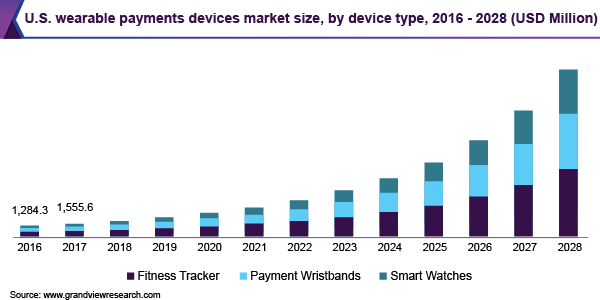
\includegraphics[width=\textwidth]{devices-market.png}
		\caption{نمودار بازار دستگاه‌های پوشیدنی از سال 2016 تا پیشبینی آن تا سال 2028\cite{markets}}
		\label{wearables}
	\end{figure}
	
	این دستگاه‌ها با قابلیت‌های پیشرفته‌ای که دارند، امکان مانیتورینگ مداوم وضعیت جسمی و روانی افراد را فراهم می‌کنند. از جمله مزایای این دستگاه‌ها می‌توان به راحتی استفاده، قابلیت حمل، و ارائه اطلاعات دقیق و به‌روز اشاره کرد. این ویژگی‌ها باعث شده‌اند تا دستگاه‌های پوشیدنی به ابزارهای ضروری در حوزه سلامت و تحقیقاتی تبدیل شوند.\\
	
	در این گزارش، از دو دستگاه پوشیدنی استفاده شده است: دستبند
	 \english{Empatica E4}
	  و بند سینه‌ای \english{Respiban}. دستبند \english{Empatica E4 } با سنسورهای مختلفی که دارد، می‌تواند اطلاعات مربوط به فعالیت‌های الکتریکی پوست، ضربان قلب، و دمای بدن را جمع‌آوری کند. بند سینه‌ای \english{Respiban} نیز با اندازه‌گیری دقیق تنفس و فعالیت قلبی، اطلاعات جامعی از وضعیت فیزیولوژیکی فرد ارائه می‌دهد. این دو دستگاه در تشخیص حالات احساسی پایه، استرس، و خوشحالی مورد استفاده قرار گرفته‌اند و داده‌های جمع‌آوری شده از آن‌ها برای تحلیل دقیق‌تر احساسات به کار گرفته می‌شوند.\\
	
	ترانسفورمرها به عنوان یکی از پیشرفته‌ترین معماری‌های مدل‌های یادگیری عمیق، انقلابی در هوش مصنوعی ایجاد کرده‌اند. این مدل‌ها با استفاده از مکانیسم توجه، توانایی تحلیل، در نظر گرفتن زمینه و پردازش موازی داده‌ها را به طور همزمان دارند که منجر به بهبود قابل توجهی در عملکرد و سرعت مدل‌های یادگیری می‌شود. ترانسفورمرها در کاربردهای مختلفی از جمله پردازش زبان طبیعی، ترجمه ماشینی، و تولید متن‌های خودکار به کار گرفته می‌شوند و توانسته‌اند دقت و کارایی مدل‌های هوش مصنوعی را به سطحی بی‌سابقه برسانند.\\
	
	در این گزارش، ما از مدل ترانسفورمر \english{BioT} که یک مدل قدرتمند برای تحلیل سیگنال‌های بیولوژیکی است، استفاده می‌کنیم. مدل \english{BioT} با بهره‌گیری از ساختار ترانسفورمر، قادر است تا اطلاعات پیچیده و متنوعی که از سیگنال‌های بیولوژیکی نظیر ضربان قلب، تنفس، و فعالیت‌های الکتریکی پوست به دست می‌آید را به طور دقیق تحلیل و تفسیر کند. این مدل به ما امکان می‌دهد تا با دقت بالاتری به تشخیص حالات احساسی پایه، استرس، و خووشحالی بپردازیم و نتایج بهتری در این حوزه به دست آوریم.\\
	
	\tableofcontents
	
	
	%---------------------
	\pagestyle{plain}
	\setcounter{page}{1}
	\pagenumbering{arabic}
	%---------------------
	
	\chapter{مجموعه داده}
	مجموعه داده \english{WESAD\cite{wesad}} یکی از کامل‌ترین ﻣﺠﻤﻮﻋﻪ ﻫﺎﻱ ﺩﺍﺩﻩ ﺑﺮﺍﻱ ﺗﺸﺨﻴﺺ ﻋﻮﺍﻃﻒ ﺍﺳﺖ. ﺑﻴﺸﺘﺮﻳﻦ ﺗﻤﺮﻛﺰ ﻭ ﺍﺳﺘﻔﺎﺩﻩ ﺍﺯ ﺍﻳﻦ ﻣﺠﻤﻮﻋﻪ ﺑﺮﺍﻱ ﺗﺸﺨﻴﺺ ﺍﺳﺘﺮﺱ ﺑﻮﺩﻩﺍﺳﺖ. ﺑﺎ ﺍﻳﻦ ﻭﺟﻮﺩ، ﺑﻪ ﺟﺰ ﻛﻼﺱ ﺍﺳﺘﺮﺱ ﻭ ﻋﺎﺩﻱ، ﺑﺮﺍﻱ ﻧﺸﺨﻴﺺ ﻛﻼﺱ ﻫﺎﻱ ﺧﻮﺷﺤﺎﻟﻲ ﻭ ﺁﺭﺍﻣﺶ ﻧﻴﺰ ﻣﻲﺗﻮﺍﻥ ﺍﺯ ﺍﻳﻦ ﺩﺍﺩﻩﻫﺎ ﺍﺳﺘﻔﺎﺩﻩ ﻧﻤﻮﺩ. ﻋﻼﻭﻩ ﺑﺮ ﺁﻥﻫﺎ، ﻫﺮ ﺷﺨﺺ پﺮﺳﺸﻨﺎﻣﻪﻫﺎﻳﻲ ﻧﻴﺰ پﺮ ﻛﺮﺩﻩ ﻛﻪ ﺍﻳﻦ ﻫﻢ ﻣﻲﺗﻮﺍﻧﺪ ﺑﺎﻋﺚ ﺧﻠﻖ ﻣﺪﻝ ﻫﺎﻱ ﺟﺪﻳﺪﻱ ﺷﻮﺩ. ﺩﻭ ﺩﺳﺘگﺎﻩ ﺍﺻﻠﻲ ﺑﺮﺍﻱ ﻓﺮﺍﻫﻢ ﺁﻭﺭﺩﻥ ﺍﻳﻦ ﺩﺍﺩﻩﻫﺎ ﻣﻮﺭﺩ ﺍﺳﺘﻔﺎﺩﻩ ﻗﺮﺍﺭ گﺮﻓﺘﻪ ﺍﻧﺪ: \textbf{1(} مچ‌بند \english{Emaptica E4} ﻪ ﺑﺴﻴﺎﺭﻱ ﺍﺯ ﺩﺍﻧﺸگﺎﻩﻫﺎﻱ ﺳﺮﺍﺳﺮ ﺩﻧﻴﺎ ﺍﺯ ﺁﻥ ﺍﺳﺘﻔﺎﺩﻩ ﻣﻲ ﻛﻨﻨﺪ\cite{empatica} و  \textbf{2(} دستگاه \english{Repiban} که یکی از پیشرفته ترین سنسورهای تحقیقاتی است که بر روی سینه نصب می‌شود\cite{respiban}.
	
	\begin{figure}
		\includegraphics[width=0.5\textwidth]{empatica.jpg}
		\hspace{1cm}
		\includegraphics[width=0.5\textwidth]{respiban.png}
		\caption{شکل راست: ساعت \english{Empatica E4} ﺭﺍ ﻧﺸﺎﻥ ﻣﻲﺩﻫﺪ. ﺍﻳﻦ ﺳﺎﻋﺖ ﺑﻪ ﺩﻟﻴﻞ ﺳﻨﺴﻮﺭﻫﺎﻱ ﻛﺎﻣﻞ، ﺯﻳﺒﺎﻳﻲ ﻭ ﺭﺍﺣﺘﻲ ﺍﺳﺘﻔﺎﺩﻩ ﻛﺎﺭﺑﺮﺩ ﺯﻳﺎﺩﻱ ﺩﺭ ﺗﺤﻘﻴﻘﺎﺕ ﺩﺍﺭﺩ. 
		شکل چپ:‌ دستگاه \english{Respiban} ﻭ ﻧﺤﻮﻩ ﻗﺮﺍﺭگﻴﺮﻱ ﺁﻥ ﺭﻭﻱ ﺳﻴﻨﻪ ﻭ ﻣﺤﻞ ﻫﺮ ﻳﻚ ﺍﺯ ﺳﻨﺴﻮﺭﻫﺎ ﺭﺍ ﻧﺸﺎﻥ ﻣﻲ ﺩﻫﺪ.}
	\end{figure}
	\section{دستگاه \english{Respiban}}
	ﺍﻳﻦ ﺩﺳﺘگﺎﻩ ﻣﻲﺗﻮﺍﻧﺪ ۶ ﻋﺎﻣﻞ ﺭﺍ ﺍﻧﺪﺍﺯﻩگﻴﺮﻱ ﻛﻨﺪ. ﻓﺮﻛﺎﻧﺲ ﻭﺭﻭﺩﻱ ﺍﻳﻦ ﺩﺳﺘگﺎﻩ ﺑﺮﺍﻱ ﻫﻤﻪ ﺳﻨﺴﻮﺭﻫﺎﻳﺶ ۷۰۰ ﻫﺮﺗﺰ ﻣﻲﺑﺎﺷﺪ. ﺳﻨﺴﻮﺭﻫﺎﻱ ﺁﻥ ﺑﻪ ﺷﺮﺡ ﺯﻳﺮ ﺍﺳﺖ:
	\begin{enumerate}
		\item مختصات‌یابی (\english{Accelerometer})
		\item نوار قلب (\english{Electrocardiogram})
		\item فعالیت الکتریکی پوست (\english{Electrodermal Activity})
		\item برق‌ماهیچه‌نگار (\english{Electromyogram})
		\item تنفس (\english{Respiration})
		\item دما (\english{Temperature})
	\end{enumerate}
	
	\section{ساعت \english{Empatica E4}}
	ﺍﻳﻦ ﺳﺎﻋﺖ ﺷﺎﻣﻞ ﺳﻨﺴﻮﺭ ﻫﺎﻱ ﻣﺨﺘﺼﺎﺕ ﻳﺎﺑﻲ، فشار خون\footnote{\english{Blood Volume Pressure}}، دما . فعالیت الکتریکی پوست است. هر یک از این ﺳﻨﺴﻮﺭﻫﺎ ﺑﺎ ﻓﺮﻛﺎﻧﺲ ﻣﺘﻔﺎﻭﺗﻲ ﺍﻧﺪﺍﺯﻩگﻴﺮﻱ ﺷﺪﻩﺍﻧﺪ. ﺩﺭ ﺟﺪﻭﻝ ﻣﻘﺪﺍﺭ ﻓﺮﻛﺎﻧﺲ ﻫﺮ ﻳﻚ ﺍﺯ ﺳﻨﺴﻮﺭﻫﺎ ﺁﻭﺭﺩﻩ ﺷﺪﻩ ﺍﺳﺖ.
	
	\begin{table}[h]
		\begin{tabular}{|c|c|}
			\hline
			سنسور & فرکانس \\
			\hline
			\english{ACC} & 32\\
			\english{BVP} & 64\\
			\english{EDA} & 4\\
			\english{Temp} & 4\\
			\hline
		\end{tabular}
	\end{table}
	\section{پرسشنامه‌ها}
	ﻋﻼﻭﻩ ﺑﺮ ﺩﻭ ﺩﺳﺘگﺎﻩ گﻔﺘﻪ ﺷﺪﻩ، ﻫﺮ ﻳﻚ ﺍﺯ ﺳﻮژﻩﻫﺎﻱ ﺁﺯﻣﺎﻳﺶ، پﺮﺳﺸﻨﺎﻣﻪ ﻫﺎﻳﻲ ﺭﺍ پﺮ ﻛﺮﺩﻧﺪ. ﺍﻳﻦ پﺮﺳﺸﻨﺎﻣﻪﻫﺎ ﺩﺭ ﺟﻬﺖ ﺩﺭﻳﺎﻓﺖ ﺍﻃﻼﻋﺎﺕ ﺑﻴﺸﺘﺮ ﺩﺭ ﻣﻮﺭﺩ ﺍﺣﺴﺎﺳﺎﺕ ﺍﺷﺨﺎﺹ ﺑﻪ ﻛﺎﺭ گﺮﻓﺘﻪ ﺷﺪﻧﺪ، ﺍگﺮچﻪ ﺩﺭ ﻫﻴچﻳﻚ ﺍﺯ ﻣﻘﺎﻻﺕ ﺑﺮﺭﺳﻲ ﺷﺪﻩ،ﻣﺤﻘﻘﺎﻥ ﺍﺯ ﺍﻳﻦ پﺮﺳﺸﻨﺎﻣﻪ ﻫﺎ ﺍﺳﺘﻔﺎﺩﻩ ﺍﻱ ﻧﻜﺮﺩﻧﺪ. ﺩﺭ ﻗﺴﻤﺖﻫﺎﻱ پﻴﺶﺭﻭ ﺍﻳﻦ پﺮﺳﺸﻨﺎﻣﻪﻫﺎ ﺭﺍ ﺑﺮﺭﺳﻲ ﻣﻲ ﻛﻨﻴﻢ:
	
	\subsection*{\english{PANAS}}
	ﺳﻮژﻩ ﻣﻲﺑﺎﻳﺴﺖ ﺑﻪ ۲۶ ﺣﺲ ﺩﺭ پﺮﺳﺸﻨﺎﻣﻪ، ﺍﺯ ۱ ﺗﺎ ۵ ﺍﻣﺘﻴﺎﺯ ﺩﻫﺪ. ﺍﻳﻦ ﺍﺣﺴﺎﺳﺎﺕ ﻋﺒﺎﺭﺗﻨﺪ ﺍﺯ: ﻓﻌﺎﻝ، پﺮﻳﺸﺎﻧﻲ، ﻋﻼﻗﻪ ﻣﻨﺪ، ﺍﻟﻬﺎﻡﺷﺪﻩ، ﺭﻧﺠﻴﺪﻩ، گﻨﺎﻫﻜﺎﺭ، ﺗﺮﺳﻴﺪﻩ، ﺩﺷﻤﻨﻲ، ﻫﻴﺠﺎﻥﺯﺩﻩ، ﻣﻐﺮﻭﺭ، ﻛﺞﺧﻠﻖ، ﻣﺸﺘﺎﻕ، ﺷﺮﻣﻨﺪﻩ، ﻫﻮﺷﻴﺎﺭ، ﻧگﺮﺍﻥ، ﻣﺼﻤﻢ، ﻣﺘﻮﺟﻪ، ﻋﺼﺒﻲ، ﻭﺣﺸﺖﺯﺩﻩ، ﺍﺳﺘﺮﺳﻲ، ﺧﺴﺘﻪ، ﺧﻮﺷﺤﺎﻝ، ﻋﺼﺒﺎﻧﻲ، ﺁﺯﺭﺩﻩﺷﺪﻥ ﻭ ﻧﺎﺭﺍﺣﺖ.
	\subsection*{\english{STAI}}
	ﺩﺭ ﺍﻳﻦ پﺮﺳﺸﻨﺎﻣﻪ، ﺳﻮژﻩ ﺑﻪ ﻫﺮ ﻳﻚ ﺍﺯ ﺳﻮﺍﻝ ﻫﺎﻱ ﺯﻳﺮ ﺍﺯ ۱ ﺗﺎ ۴ ﻧﻤﺮﻩ ﻣﻲ ﺩﻫﺪ:
	\begin{enumerate}
		\item ﻣﻦ ﺍﺣﺴﺎﺱ ﺭﺍﺣﺘﻲ ﻣﻲ ﻛﻨﻢ
		\item ﻣﻦ ﺍﺣﺴﺎﺱ ﻧگﺮﺍﻧﻲ ﻣﻲ ﻛﻨﻢ
		\item ﻣﻦ ﻋﺼﺒﻲ ﻫﺴﺘﻢ
		\item ﻣﻦ ﺭﻳﻠﻜﺲ ﻫﺴﺘﻢ
		\item ﻣﻦ ﺍﺣﺴﺎﺱ ﺩﻟﻮﺍپﺴﻲ ﻣﻲ ﻛﻨﻢ
		\item ﻣﻦ ﺍﺣﺴﺎﺱ ﺭﺿﺎﻳﺖ ﻣﻲ ﻛﻨﻢ
	\end{enumerate}
	\subsection*{\english{SAM}}
	ﺍﻳﻦ ﺗﺴﺖ ﺷﺪﺕ ﻭ ﺧﻮﺏ ﻳﺎ ﺑﺪ ﺑﻮﺩﻥ ﺍﺣﺴﺎﺳﺎﺕ ﺭﺍ ﻣﻲ ﺳﻨﺠﺪ. ﺷﺨﺺ ﺩﻭ ﺳﻮﺍﻝ ﺭﺍ ﺩﺭ ﻣﻘﻴﺎﺱ ۱ ﺗﺎ ۹ پﺎﺳﺦ ﻣﻲ ﺩﻫﺪ: \textbf{1(} ﺣﺲ ﻣﻦ چقدر ﺧﻮﺏ ﺍﺳﺖ ﻭ \textbf{2(} ﺷﺪﺕ ﺍﻳﻦ ﺣﺲ چقدر ﺍﺳﺖ.
	\subsection*{\english{SSSQ}}
	ﺍﻳﻦ ﺗﺴﺖ ﻛﻪ ﻛﻮﺗﺎﻩﺷﺪﻩ ﺗﺴﺖ ﺍﺳﺘﺎﻧﺪﺍﺭﺩ \english{SSSQ} ﺍﺳﺖ، ﺩﺭ ﺯﻣﺎﻥﻫﺎﻱ ﺍﺳﺘﺮﺱ ﺍﺯ ﺷﺮﻛﺖ ﻛﻨﻨﺪگﺎﻥ گﺮﻓﺘﻪ ﺷﺪﻩ ﺍﺳﺖ. پﺮﺳﺶﺷﻮﻧﺪگﺎﻥ ﺑﻪ ﺳﻮﺍﻝﻫﺎﻱ ﺯﻳﺮ ﺍﺯ ۱ ﺗﺎ ۵ ﻧﻤﺮﻩ ﻣﻲ ﺩﻫﻨﺪ:
	\begin{enumerate}
		\item ﻣﻦ ﻣﺘﻌﻬﺪ ﺑﻪ ﺭﺳﻴﺪﻥ ﺑﻪ ﺍﻫﺪﺍﻑ ﻋﻤﻠﻜﺮﺩﻱﺍﻡ ﻫﺴﺘﻢ
		\item ﻣﻦ ﻣﻲﺧﻮﺍﻫﻢ ﺩﺭ ﺍﻳﻦ ﻛﺎﺭ ﻣﻮﻓﻖ ﺷﻮﻡ
		\item ﻣﻦ ﺍﻧگﻴﺰﻩ ﺑﺮﺍﻱ ﺍﻧچﺎﻡ ﺍﻳﻦ ﻛﺎﺭ ﺭﺍ ﺩﺍﺭﻡ
		\item ﻣﻦ ﺧﻮﺩﻡ ﺭﺍ ﺑﺮﻭﺯ ﻣﻲ ﺩﻫﻢ
		\item ﻣﻦ ﻧگﺮﺍﻥ ﺗﻔﻜﺮﺍﺕ ﺩﻳگﺮﺍﻥ ﺩﺭ ﻣﻮﺭﺩ ﺧﻮﺩﻡ ﻫﺴﺘﻢ
		\item ﻣﻦ ﻣﺘﻮﺟﻪ ﺗﺎﺛﻴﺮﻱ ﻛﻪ ﺭﻭﻱ ﺑﻘﻴﻪ ﻣﻲ گﺬﺍﺭﻡ ﻫﺴﺘﻢ
	\end{enumerate}
	\section{طبقه‌بندی}
	ﺍﻳﻦ ﻣﺠﻤﻮﻋﻪﺩﺍﺩﻩ ﻋﻮﺍﻃﻒ ﺍﻧﺴﺎﻥ ﻫﺎﻱ ﻣﻮﺭﺩ ﺑﺮﺭﺳﻲ ﺭﺍ ﺩﺭ ۴ ﻃﺒﻘﻪ ﺷﻨﺎﺳﺎﻳﻲ ﻛﺮﺩﻩ ﺍﺳﺖ: 1) حالت معمولی\footnote{\english{baseline}}، 2) استرس، 3) خوشحالی \footnote{\english{Amusement}}و 4) آرامش\footnote{\english{Meditated}}.
	
	\begin{table}[h]
		\begin{tabular}{|c|c|}
			\hline
			
			سوژه & ثانیه‌های مفید \\
			\hline
			2 & 2884\\
			3 & 2930\\
			4 & 2965\\
			5 & 3006\\
			6 & 2984\\
			7 & 2983\\
			8 & 3000\\
			9 & 2985\\
			10 &3068\\
			11 &3014\\
			13 &3016\\
			14 &3016\\
			15 &3022\\
			16 &3008\\
			17 &3002\\
			\hline
		\end{tabular}
		\caption{ثانیه‌های مفید هر یک از سوژه‌ها}
		\label{classes}
		
	\end{table}
	در جدول\ref{classes} ثانیه های مفید هر یک از سوژه‌ها آورده شده است. منظور از ثانیه‌های مفید، آنهایی است که کلاس های آنها حالت پایه، استرس، خوشحالی و یا آرامش است. در دادگان دو کلاس بی‌نام دیگر وجود دارد که آنها میباست حذف شوند.
	
	ﻛﻼﺱگذﺍﺭﻱ ﺩﺭ ﺑﻴﺸﺘﺮﻳﻦ ﻓﺮﻛﺎﻧﺲ ﻣﻤﻜﻦ (۷۰۰) ﺻﻮﺭﺕ گرﻓﺘﻪ ﻭ ﺑﺮﺍﻱ ﻫﺮ ﻳﻚ ﺍﺯ ﺳﻨﺴﻮﺭﻫﺎ ﺑﺮﺍﻱ ﺩﺳﺘﻴﺎﺑﻲ ﺑﻪ ﻛﻼﺱ ﻣﻮﺭﺩﻧﻈﺮ ﺑﺎﻳﺪ ﺁﻥ ﺭﺍ ﺑﻪ ﻓﺮﻛﺎﻧﺲ ﺁﻥ ﺳﻨﺴﻮﺭ ﺗﺒﺪﻳﻞ ﻛﻨﻴﻢ.
	
	
	\chapter{کارهای مشابه}
	کارهای زیادی با استفاده از این مجموعه داده برای تشخیص عواطف صورت گرفته است. گرجه این دادگان در 4 کلاس گردآوری شده، بیشتر کارها 2کلاسه یا 3کلاسه (حالت عادی، استرس و خوشحالی) هستند. همچنین از پرسشنامه‌های موجود در دادگان بهره جندانی برده نشده‌است.
	
	
	در جدول \ref*{related} کارهای مشابه که از این دادگان استفاده کردند آورده شده‌است. 
	\begin{table}[h]
		\begin{tabular}{|p{0.35\linewidth}|p{0.25\linewidth}|p{0.2\linewidth}|p{0.2\linewidth}|}
			\hline
			نام کار & سیگنال‌ها & پنجره & عملکرد \english{f-1}\\
			\hline
			\english{Introducing WESAD, a Multimodal Dataset for Wearable
				Stress and Affect Detection\cite{wesad}} & \english{Extracted features from all the signals} &  پنجره : 60 ثانیه، قدم:  $\text{1}/\text{4}$ ثانیه  & \english{2class: 91.47, 3class: 72.51}\\
			\hline
			\english{Transformer-based Self-supervised Multimodal
				Representation Learning for Wearable Emotion
				Recognition\cite{transformer1}} & \english{Wrist BVP, EDA, and Temp} & پنجره : 60  ثانیه (4 هرتز)، قدم:  $\text{1}/\text{4}$ ثانیه & 
				\english{2class: 93.69, 3class: 82.01}\\
			\hline
			\english{Affective State Recognition with Convolutional Autoencoders\cite{convAE1}} & \english{All the signals} &‌ پنجره: 1 ثانیه‌، قدم: 1 ثانیه & \english{3class: 82.82}\\
			\hline
			\english{Stress Detection by Machine Learning and Wearable Sensors\cite{art2021}} &‌ \english{Manual features from all the chest signals} &
			 پنجره: 10 ثانیه، قدم: 10 ثانیه & \english{2class: 83.34, 3class: 65.73}\\
			\hline
			\english{A Transformer Architecture for Stress Detection from ECG\cite{behnam2021}} & \english{ECG} & پنجره: 30 ثانیه‌، قدم: 1 ثانیه &‌ \english{2class: 83.3}\\
			
			\hline
		\end{tabular}
		\caption{کارهای مشابه بر روی دادگان \english{WESAD}}
		\label{related}
		
	\end{table}
	
	\section{روش شناسی}
	در ادادمه به بررسی روش استفاده شده در هر یک از کارهای نام برده شده می‌پردازیم:
	\begin{itemize}
		\item [$\bullet$]
		\english{Introducing WESAD, a Multimodal Dataset for Wearable
			Stress and Affect Detection\cite{wesad}}:\\
		
		در اینجا از استخراج ویژگی‌های پیچیده‌ای استفاده گردیده‌است. برای \english{ACC} میانگین و انحراف معیار برای هر یک از ابعاد شناسایی و با هم جمع شده و علاوه بر آن نقطه اوج هر یک نیز محاسبه گردیده.\\
		از سیگنال‌های \english{ECG} و \english{BVP} میانگین و واریانس آنها و همجنین از نقاط پیک آنها ضربان قلب و از زمان های ضربان قلب، تغییرات آن\footnote{\english{Heart Rate Variability}} به دست می‌آید.\\
		برای \english{EDA} ابتدا یک فیلتر پایین‌گذر\footnote{\english{low pass filter}} 5 هرتزی بر روی آن اعمال و میانگین و واریانس محاسبه می‌شود. همچنین دو بخش تونیک و فازیک این سیگنال (به نام‌های \english{Skin Conductance Level} و \english{Skin Conductance Response}) با توجه به کار \cite{eda} استخراج شدند.\\
		بر روی سیگنال \english{EMG} ابتدا یک فیلتر بالاگذر\footnote{\english{high pass filter}} اعمال و سپس نقاط پیک شناسایی شدند و چندین ویژگی دیگر با توجه به کار \cite{emg} استخراج شدند.\\
		برای \english{Resp} ایتدا یک فیلتر میان‌گذر
		 \footnote{\english{band pass filter}} بر روی آن اعمال شدند. پیک‌ها شناسایی و میانگین و واریانس دم و بازدم‌ها محاسبه شدند. علاوه بر آنها نسبت دم به بازدم، حجم تنفس، نرخ تنفس و مدت زمان تنفس نیز محاسبه گردیدند.\\
		برای دما، میانگین و واریانس و بیشینه و کمینه و شیب آن محاسبه گردیده بود.\\
		برای انجام کلاسیفیکیشن، 5 روش دسته‌بندی
		\emph{درخت تصمیم}\footnote{\english{Decision Tree}}
		 \emph{جنگل تصادفی}\footnote{\english{Random Forest}}،
		‌ \emph{\english{k}-همسایه-نزدیک}\footnote{\english{K-Nearest-Neighbor}}، 
		\emph{تحلیل تشخیصی خطی}\footnote{\english{Linear Discriminant Analysis}} و
		\emph{\english{AdaBoost}} 
		استفاده شدند.
		\item [$\bullet$]
		\english{Transformer-based Self-supervised Multimodal
			Representation Learning for Wearable Emotion
			Recognition\cite{transformer1}}:\\
		
		ابتدا چندین تبدیل روی هر پنجره اتفاق می‌افتد:
		\begin{enumerate}
			\item 
			\textbf{جایگشت:}
			قسمت‌های مختلف پنجره حدا شده و سپس با جایگشتی دیگر به هم چسبانده می‌شوند.
			\item 
			\textbf{پیچ و تاب زمانی: }
			پنجره سیگنال به \english{n} قسمت تقسیم شده و نیمی از آنها منبسط و نیمی دیگر منقبض می‌شوند.
			\item 
			\textbf{برش: }
			با تقسیم پنجره به \english{n} قسمت، یکی را حذف کرده و دوباره نمونه‌گیری می‌کنیم.
		\end{enumerate}
		\begin{figure}[h]
			\includegraphics[width=\textwidth]{self_super_trans.png}
			\caption{
				معماری مدل مقاله \cite{transformer1}. مدل ترانسفورمر اصلی از یک توجه چندکله‌‌ای (\english{Multi-Head Attention})  و سپس نرمال‌ساز لایه (\english{Layer Normalization})  و سپس یک لایه کامل‌متصل (\english{Fully Connected}) و دوباره یک نرمال‌ساز لایه دیگر.
			}
			\label{trans1model}
		\end{figure}
		
		معماری مدل در شکل \ref{trans1model} آورده شده‌است.	مرحله آموزش شامل دو مرحله بوده. اول پیش‌آموزش آن روی دادگان \english{PRESAGE}\cite{presage} انجام می‌شود. در مرحله دوم از انکودر مدل پیش‌اموزش داده شده برای کلاسیفیکیشن استفاده می‌شود.
		\item [$\bullet$]
		\english{Affective State Recognition with Convolutional Autoencoders\cite{convAE1}}:\\
		3 اتوانکودر مورد استفاده قرار می‌گیرند. یکی برای سیگنال‌های سینه‌ای که 80 ویژگی هدف آن است. برای سیگنال \english{BVP} مچ هم یک اتوانکودر که 40 ویژگی را استخراج می‌کند. در انتها برای سیگنال‌های مچی \english{EDA} و دما نیز یکی دیگر که تنها 4 ویژگی را تحویل دهد.\\
		
		در نهایت این 124 ویژگی با هم تجمیع شده و به دسته‌یندی‌کننده \english{SVM} خورانده می‌شود تا دسته بندی را انجام دهد.
		
		
		\item [$\bullet$]
		\english{Stress Detection by Machine Learning and Wearable Sensors\cite{art2021}}:\\
		در این کار بیشینه، کمینه، میانگین و انحراف معیار پنجره‌های 10 ثانیه‌ای بدون اشتراک به دست آورده شده است و سپس با بهره‌گیری از 5 روش دسته‌بندی \emph{جنگل تصادفی}،
		‌ \emph{\english{k}-همسایه-نزدیک}، 
		\emph{تحلیل تشخیصی خطی}،
		 \emph{\english{AdaBoost}} 
		و \emph{ماشین بردار پشتیبان}\footnote{\english{Support Vector Machine}}،
		 آن‌ها را دسته‌بندی کرده‌اند.
		\item [$\bullet$]
		\english{A Transformer Architecture for Stress Detection from ECG\cite{behnam2021}}:\\
		
		
	\end{itemize} 
	\chapter{پیش‌پردازش}
	در بخش‌های پیش‌رو در مورد کارهای مورد نیاز برای آماده‌سازی داده‌ها برای آموزش مدل‌ها بحث می‌کنیم
	
	\section{ساختار مجموعه داده}
	در دادگان \english{WESAD} ﺩﺍﺩﻩﻫﺎﻱ ﺗﺠﻤﻴﻊﺷﺪﻩ ﻭ ﻫﻤگﺎﻡﺷﺪﻩ ﺭﺍ ﺑﺮﺍﻱ ﻫﺮ ﺳﻮژﻩ ﺩﺭ ﻳﻚ ﻓﺎﻳﻞ \english{pkl} ﻓﺮﺍﻫﻢ ﺁﻭﺭﺩﻩﺍﻧﺪ. ﺍﻳﻦ ﻓﺎﻳﻞ ﻳﻚ ﺩﻳﻜﺸﻨﺮﻱ ﺑﻪ ﺻﻮﺭﺕ ﺯﻳﺮ ﺍﺳﺖ.
	
	\begin{figure}
		\lr{
			\dirtree{%
				.1 `Sx.pkl`.
				.2 subject.
				.2 label.
				.2 signal.
				.3 chest.
				.4 ACC.
				.4 ECG.
				.4 EMG.
				.4 EDA.
				.4 Temp.
				.4 Resp.
				.3 wrist.
				.4 ACC.
				.4 BVP.
				.4 EDA.
				.4 TEMP.
			}
		}
		
		\caption{ساختار اولیه دادگان \english{WESAD}}
		\label{fig:struct}
		
	\end{figure}
	
	آرایه \english{label} و تمام آرایه‌های سنسورهای \english{chest}، به طول 4,545,100 هستند، که همه  700$Hz$ در طول 6493 ثانیه هستند. آرایه‌های \english{ACC} و \english{BVP} به ترتیب 32 و 64 هرتز و دو سیگنال دیگر هر دو 4 هرتز هستند.\\
	
	\section{تمیزسازی دادگان}
	همانطور که در بالا گفته شد، برخی کلاس های داده بلااستفاده هستند. در قدم اول این‌ها حذف می‌شوند و تنها ثانیه‌های مفید باقی می‌مانند. سپس برای زیباسازی ساختار ذخیره داده، آن را به شکل\ref{fig:struct2} تغییر می‌دهیم.
	
	\begin{figure}
		\lr{
			\dirtree{%
				.1 `Sx\_n0.pkl`.
				.2 label.
				.2 chest\_ACC.
				.2 chest\_ECG.
				.2 chest\_EMG.
				.2 chest\_EDA.
				.2 chest\_Temp.
				.2 chest\_Resp.
				.2 wrist\_ACC.
				.2 wrist\_BVP.
				.2 wrist\_EDA.
				.2 wrist\_TEMP.
			}
		}
		
		\caption{ساختار دادگان پس از تغییر}
		\label{fig:struct2}
		
	\end{figure}
	
	\chapter{آموزش}
	\section{مدل \english{BioT}}
	مدل \english{BioT} برای کار با داده های \english{EEG} طراحی و ساخته شده‌است. اما همانطور که از نام آن پیداست (\english{Bio Transformer}) از آن می‌توان برای انواع سیگنال های حیاتی بهره گرفت. در شکل \ref{biot} ساختار این مدل را مشاهده می‌کنید. در نیم تصویر بالا،‌ ماژول توکنایز کردن سیگنال‌هاست، که با انجام دوباره نمونه‌گیری\footnote{\english{resampling}}، نرمال کردن، توکنایز کردن و تخت کردن\footnote{\english{flattening}}، آن را تبدیل به جملات می‌کند.
	
	\begin{figure}[h]
		\includegraphics[width=\textwidth]{biot.png}
		\caption{معماری شبکه \english{BioT}}
		\label{biot}
		
	\end{figure}
	
	سپس تعامل بین این جملات با استفاده از ماژول ترنسفورمر خطی (نیم‌تصویر پایین) یاد گرفته می‌شوند. این مدل به صورت با نظارت می‌تواند داده‌های مختلف کامل و ناقص را برای پیش‌آموزش و \english{fine-tuning} بپیذیرد.
	
	\section{ساختار مدل}
	مدل از دو بخش انکودر و سر کلاسیفیکیشن\footnote{\english{Classification Head}} تشکیل شده‌است.\\
	
	سر کلاسیفیکیشن از یک تابع فعالساز \english{ELU}\footnote{\english{Exponential Linear Unit}} و یک لایه خطی تشکیل شده‌است که با تبدیل $xA^T + b$ انکودینگ ساخته شده را به یک وکتور با اندازه تعداد کلاس‌ها می‌برد که بیانگر احتمال این است که آن ورودی در هر کدام از آن کلاس‌ها باشد.\\
	
	بخش انکودر نیز ابتدا یک امبدینگ اولیه ساخته و سپس آن را به ترانسفورمر داده تا برای پنجره مورد نظر یک امبدینگ نهایی بسازد. در قسمت پیش‌رو به تفصیل این دو بخش توضیح داده شده‌اند.
	\subsection{امبدینگ اولیه}
	برای محاسبه یک امبدینگ اولیه، برای هر یک از کانال‌ها، فرایند زیر محاسبه می‌گردد:
	\begin{enumerate}
		\item 
		بر روی سیگنال آن کانال، \english{STFT}\footnote{\english{Short-Time Fourier Transform}} اعمال می‌گردد.
		\item 
		سپس بر روی آن \english{Patch Frequency embedding} صورت می‌گردد. برای این امر ابتدا یک جایگشت بر روی ابعاد سیگنال اعمال شده و سپس با یک تبدیل خطی\footnote{\english{Linear}} آن را به ابعاد 256 می‌بریم.
		\item 
		در نهایت انکودینگ مکانی\footnote{\english{Positional Encoding}} بر آن افزوده می‌شود. 
	\end{enumerate}
	
	پس از انجام این فرایندها بر روی سیگنال‌های هر کانال آن ها را با هم میانگین می‌گیریم و امبدینگ اولیه آماده می‌شود.
	\subsection{بخش ترانسفورمر}
	بخش انکودر نیز ابتدا یک امبدینگ از ورودی ساخته و سپس آن را به یک ترانسفورمر با توجه خطی\footnote{\english{Linear Attention Transformer}} پاس می‌دهد. سپس خروجی ترانسفورمر که یک تنسور به ابعاد
	$(batch_size, combined_seq_len, emb_size)$
	است را با میانگین‌گیری در بعد اول تبدیل به تنسوری به ابعاد
	 $(batch_size, emb_size)$
	 می‌کنیم، تا برای هر پنجره از هر سیگنال‌ها به یک امبدینگ برسیم که برگرفته از اطلاعات کل پنحره در طول زمان است.\\
	 
	
	\section{مراحل خوراندن داده به مدل}
	برای آماده‌سازی داده خام و خوراندن آن به مدل \english{BioT} می‌بایست چندین کار انجام داد.\\
	
	پس از تمیزسازی دادگان که در بالا گفته شد، برای هر سوژه یک فایل \english{pickle} ساخته می‌شود که مجموع 15 فایل می‌شود. هر یک از این فایل‌ها یک دیکشنری به فرمت شکل \ref{fig:struct2} است، که هر یک از آنها یک تنسور است. طول تنسور تک بعدی \english{label} 4 برابر ثانیه‌های آن سوژه و ابعاد باقی تنسورهای سیگنال‌ها برابر
	
	$(\text{4برابر ثانیه‌ها}, \text{تعداد کانال‌ها}, \text{فرکانس سیگنال})$
	
	است.\\
	علت 4 برابر شدن ثانیه‌ها استفاده از ربع ثانیه به عنوان واحد زمانی است.  همچنین تعداد کانال‌ها برای همه به جز \english{ACC} برابر 1 است.\\
	
	
	\subparagraph{تغییر فرکانس}
	
	فرکانس مناسب برای مدل \english{BioT} برابر 200 هرتز است. بنابرین برای هر یک از سیگنال‌ها فرکانس سیگنال را به 200 تبدیل می‌کنیم. همچنین در کانال‌های مختلف میانگین می‌گیریم (در حقیقت این کار به جز بر \english{ACC} بر سیگنال دیگری تاثیری ندارد). در نهایت ابعاد هر یک از سیگنال‌ها به شکل 
	
	$(\text{4برابر ثانیه‌ها}, \text{200})$
	
	در می‌آید.\\
	
	برای تغییر فرکانس دو تابع مختلف استفاده کردیم:
	
	\begin{enumerate}
		\item 
		یکی از بهترین روش‌ها برای این کار بهره‌گیری از \english{PCA} است. این روش را تنها برای سیگنال‌های سینه می‌شود استفاده کرد، چراکه \english{PCA} تنها می‌تواند ابعاد را کم کند و سیگنال‌های مچ‌بند در بیشترین حالت 64 هرتز هستند.
		
		\item
		 روش دیگر استفاده از تابع \english{resample} از پکیج \english{scipy} بود. این تابع از متود فوریه برای تبدیل فرکانس یک سیگنال استفاده می‌کند. از این روش می‌توان برای همه سیگنال‌ها استفاده کرد.
	\end{enumerate}
	
	\subparagraph{نرمال‌سازی}
	
	با توجه به خود مدل \english{BioT}، نرمال‌سازی به این صورت انجام می‌شود که سیگنال‌ها بر چندک 95-صدم تقسیم می‌شود.
	
	\subparagraph{تقسیم دادگان}
	
	همانند تمامی مقالات و کارهای انجام شده بر روی این دادگان، ما هم از روش  \english{LOSO} استفاده می‌کنیم. بدین ترتیب به ازای هر یک از سوژه‌‌ها،‌ آن را به عنوان تست و از 14 تای باقی‌مانده،‌ 10 تا را به عنوان داده آموزشی و 4 تای باقی‌مانده را به عنوان داده \english{validation} استفاده می‌کنیم.
	
	\section{استخراج ویژگی‌ها}
	برای تبدیل داده به فرم مناسب برای آموزش مدل‌های ماشین لرنینگ، یکی از روش‌های پرکاربرد و محبوب، استخراج ویژگی از پنجره‌های سری زمانی است. در کارهای مختلف از پنجره‌های با طول‌های متفاوت استفاده می‌کنند. برای مثال در \cite{art2020} از پنجره‌هایی به طول 1 ثانیه، 10 ثانیه\cite{art2021}، و حتی 30 ثانیه\cite{behnam2021} استفاده کردند. در مورد آخر، یکی از علل طول زیاد پنجره به دلیل استفاده از مدل \english{transformer} و بهره‌گیری از زمینه\footnote{\english{context}} است.\\
	
	\section{سنجش}
	برای سنجش مدل همانند تمامی کارهای بررسی شده، از روش \english{LOSO}\footnote{\english{Leave-One-Subject-Out}} و معیار \english{F-1} استفاده می‌کنیم.
	\subparagraph{\english{LOSO}}
	در روش \english{LOSO} هر مرتبه یک سوژه را به عنوان تست و سوژه‌های دیگر برای آموزش و صحت‌سنحی استفاده می‌کنیم. در انتها نمره‌های به دست آمده را میانگین گرفته و نمره  نهایی را تعیین می‌کنیم. در شکل \ref{loso} این روش به صورت گرافیکی نمایان شده‌است.
	\begin{figure}[h]
		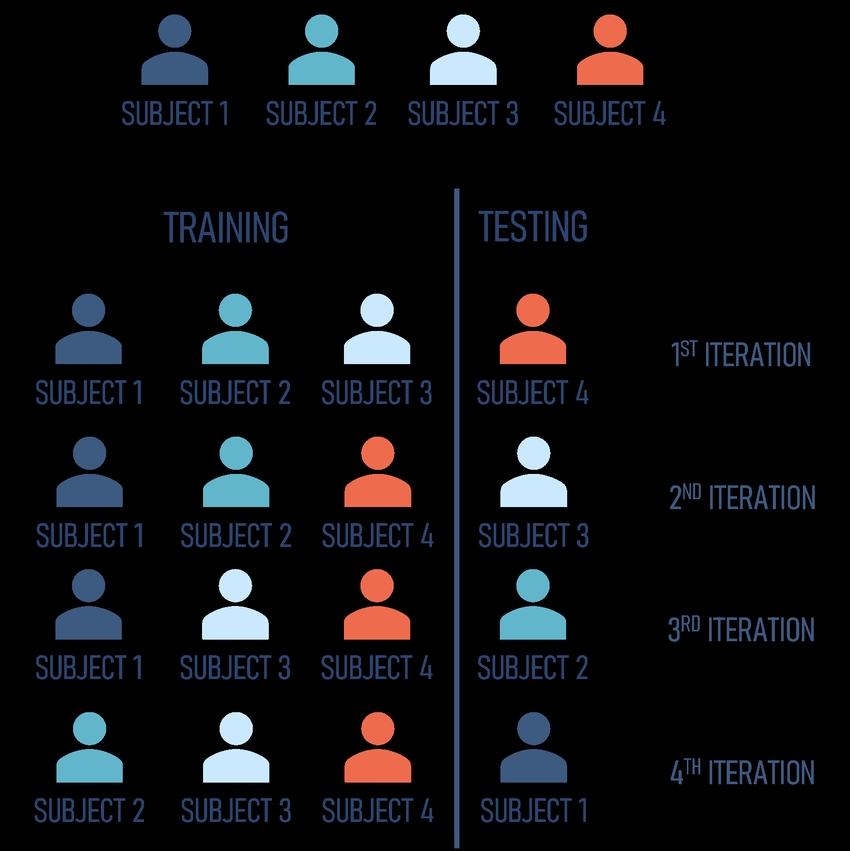
\includegraphics[width=0.8\textwidth]{loso.png}
		\caption{شکل توضیح دهنده روش \english{LOSO}}
		\label{loso}
	\end{figure}
	
	\subparagraph{\english{F-1}}
	یکی از معیارهای پرکاربرد در سنجش مدل‌های هوش مصنوعی امتیاز \english{F-1} است. چراکه در آن هم دقت و هم صحت در نظر گرفته می‌شوند و این می‌تواند مدل‌ها را بهتر از معیار دقت به تنهایی ارزیابی کند. این نمره از میانگین هارمونیک دقت و فراخوانی به دست می‌آید که در رابطه زیر نمایش داده شده‌است:
	\begin{align*}
		\text{\english{F-1}} &= \frac{2}{\frac{1/\text{\english{Precision}}}{1/\text{\english{Recall}}}}\\
		&=\frac{2\times \text{\english{Precision}}\times \text{\english{Recall}}}{\text{\english{Precision}} + \text{\english{Recall}}}
	\end{align*}

	\chapter{نتایج}
	\section{2 کلاسه}
	برای مقایسه آن با هر یک از کارها، این مدل را با استفاده از سیگنال‌ها و پنجره‌های هر یک از کارها مقایسه می‌کنیم.\\
	در ابتدا مقایسه را 2کلاسه (استرس و غیر استرس) انجام می‌دهیم. در جدول \ref{compare1} نتایج با دو روش اول که پنجره‌های یکسانی داشتند مقایسه شدند. میانگین \english{f1-score} برابر 91 درصد شد که دقتی نسبتا خوب محسوب می‌شود.  به دلیل محدودیت‌های محاسباتی به جای قدم‌های ربع ثانیه‌ای از قدم‌های 6 ثانیه‌ای استفاده شد که اینگونه تعداد داده‌های آموزش به نسبت کار \cite{transformer1} که بهترین کار بوده، بسیار کمتر (حدودا 25 برابر) بوده ولی با این حال دقت تنها 2 درصد کمتر بوده که با کاهش اندازه قدم‌ها این درصد نیز بهتر خواهد شد.
	
	\begin{table}[h]
		\begin{tabular}{|c|c|c|}
			
			\hline
			سوژه & امتیاز \english{F-1} & \english{Accuracy}\\
			\hline
			2&$0.78$&$0.70$\\
			3&$0.82$&$0.79$\\
			4&$0.90$&$0.88$\\
			5&$0.96$&$0.96$\\
			6&$0.90$&$0.89$\\
			7&$0.82$&$0.80$\\
			8&$0.84$&$0.80$\\
			9&$0.80$&$0.73$\\
			10&$0.96$&$0.96$\\
			11&$0.90$&$0.90$\\
			13&$0.96$&$0.96$\\
			14&$0.70$&$0.73$\\
			15&$0.96$&$0.96$\\
			16&$0.98$&$0.98$\\
			17&$0.70$&$0.72$\\
			\hline
			مجموع&$0.91$&$0.93$\\
			\hline
		\end{tabular}
		\caption{
			نتایج کلاسیفیکیشن 2کلاسه با مدل \english{BioT} با پنجره 60 ثانیه و قدم‌های ربع ثانیه‌ای. سیگنال های \english{BVP}، \english{EDA} و دمای مج استفاده شدند.}
		\label{compare1}
		
	\end{table}
	
	
	\section{3 کلاسه}
	در قدم بعدی این مدل را برای 3 کلاس تست کردیم. 3 کلاس عبارتند از استرس،‌ خوشحالی و عادی. در ادامه این کار را با سیگنال‌های مختلف بررسی کردیم:\\
	
	\subsection{سیگنال‌های سینه‌ای}
	\begin{table}[h]
		\begin{tabular}{|c|c|c|}
			\hline
			سوژه & امتیاز \english{F-1} & \english{Accuracy}\\
			\hline
			2&$0.75$&$0.64$\\
			3&$0.54$&$0.57$\\
			4&$0.85$&$0.78$\\
			5&$0.23$&$0.18$\\
			6&$0.77$&$0.67$\\
			7&$0.54$&$0.59$\\
			8&$0.85$&$0.78$\\
			9&$0.77$&$0.67$\\
			10&$0.77$&$0.67$\\
			11&$0.77$&$0.67$\\
			13&$0.85$&$0.78$\\
			14&$0.77$&$0.67$\\
			15&$0.85$&$0.78$\\
			16&$0.85$&$0.81$\\
			17&$0.77$&$0.67$\\
			\hline
			مجموع&$0.78$&$0.71$\\
			\hline
		\end{tabular}
		\caption{همانند \ref{compare1}، با تفاوت اینکه در اینجا 3 کلاس را مقایسه کردیم. در اینجا تمام سنسورهای سینه و به وسیله \english{PCA} بررسی شده‌اند.}
		\label{compare2}
		
	\end{table}
	
	اولین آزمایش  که نتایج آن در جدول\ref{compare2} آمده، را با بهره‌گیری از \english{PCA} و سیگنال‌های سینه انجام دادیم. نتایج آن به نسبت کار \cite{art2021} که از سیگنال‌های سینه بهره برده بود، حدود 10\% امتیاز \english{F-1} بهتری داشت.\\
	
	سپس آزمایش مشابهی را این بار با \english{resample} به جای \english{PCA} انجام دادیم. بدین صورت که به جای اینکه اجزای اصلی پنجره را به دست آوریم، یک نمونه پریودیک به وسیله فوریه از آن بگیریم و از آن استفاده کنیم.\\
	
	\begin{table}[h]
		\begin{tabular}{|c|c|c|}
			\hline
			سوژه & امتیاز \english{F-1} & \english{Accuracy}\\
			\hline
			2&$0.75$&$0.64$\\
			3&$0.77$&$0.67$\\
			4&$1.0$&$1.0$\\
			5&$1.0$&$1.0$\\
			6&$0.85$&$0.81$\\
			7&$0.77$&$0.74$\\
			8&$0.69$&$0.74$\\
			9&$0.85$&$0.85$\\
			10&$0.77$&$0.67$\\
			11&$0.77$&$0.67$\\
			13&$1.0$&$1.0$\\
			14&$0.46$&$0.46$\\
			15&$0.85$&$0.86$\\
			16&$0.92$&$0.92$\\
			17&$0.69$&$0.63$\\
			\hline
			مجموع&$0.87$&$0.83$\\
			\hline
		\end{tabular}
		\caption{نتایج 3 کلاسه با تنظیمات مشابه \ref{compare2} با تفاوت اینکه به جای استفاده از 
			\english{PCA}
			، از
			 \english{resample}
			 استفاده شده‌است.}
		\label{compare3}
	\end{table}
	
	در جدول \ref{compare3} که از \english{resample} استفاده شده،‌ نتایج به مراتب بهتری گرفتیم و \english{ّF-1 score} حدود 9\% بهتر شد. این پیشرفت قابل توجه به معنای آن است که تابع بهره گرفته از فوریه \english{resample} بسیار بهتر \english{PCA} عمل می‌کند.\\
	در نهایت با سیگنال‌های سینه به تنهایی، در امتیاز \english{F-1} به 87\% رسیدیم که از مدل تمام سینه \cite{art2021} که از مدل‌های کلاسیفیکیشن کلاسیک مانند  حدود 20\% بهتر است
	
	\subsection{سیگنال‌های مچ}
	در جدول \ref{compare4} نتایح برای سیگنال‌های مچ که عبارتند از \english{BVP}، \english{ٍEDA} و دما، آورده شده‌است.\\
	
	\begin{table}[h]
		\begin{tabular}{|c|c|c|}
			\hline
			سوژه & امتیاز \english{F-1} & \english{Accuracy}\\
			\hline
			2&$0.92$&$0.92$\\
			3&$0.77$&$0.75$\\
			4&$0.85$&$0.78$\\
			5&$0.85$&$0.78$\\
			6&$0.85$&$0.81$\\
			7&$0.85$&$0.85$\\
			8&$1.0$&$1.0$\\
			9&$0.85$&$0.81$\\
			10&$0.77$&$0.67$\\
			11&$0.77$&$0.67$\\
			13&$1.0$&$1.0$\\
			14&$0.23$&$0.087$\\
			15&$1.0$&$1.0$\\
			16&$1.0$&$1.0$\\
			17&$0.69$&$0.63$\\
			\hline
			مجموع&$0.89$&$0.84$\\
			\hline
		\end{tabular}
		\caption{
			نتایج کلاسیفیکیشن 3کلاسه با استفاده از سیگنال‌های مچ. برای تغییر فرکانس از \english{resample} بهره گرفته شد. باقی تنظیمات مانند قبل است.
			}
		\label{compare4}
	\end{table}
	
	با استفاده از این سیگنال‌ها به امتیاز \english{F-1} برابر 0.89 رسیدیم که نتیجه کمی بهتری نسبت به سیگنال‌های سینه داشتیم. به علت \english{resample} کردن سیگنال‌‌ها، مزیت 700هرتزی بودن سیگنال‌های سینه کمرنگ شد. همین امر باعث این شد که اطلاعات بیشتری از سیگنال‌های مچ دست نخورده باقی بماند و همین مسبب دقت نسبتا بهتر در اینجا بوده‌است.\\
	
	\subsection{جفت سیگنال‌ها}
	
	برای بهتر شدن نتایج، اطلاعات بیشتری را به مدل دادیم و بدین ترتیب هم از سیگنال‌های سینه و هم مچ استفاده کردیم تا از مزایای هر دو استفاده کنیم و زمینه غنی‌تری را برای مدل فراهم آوریم تا نتیجه بهتری را شاهد باشیم. در جدول \ref{compare5} نتایح حاصله آورده شده‌است.\\
	
	\begin{table}[h]
		\begin{tabular}{|c|c|c|}
			\hline
			سوژه & امتیاز \english{F-1} & \english{Accuracy}\\
			\hline
			2&$0.75$&$0.73$\\
			3&$0.69$&$0.63$\\
			4&$0.92$&$0.91$\\
			5&$0.92$&$0.91$\\
			6&$0.85$&$0.86$\\
			7&$0.85$&$0.85$\\
			8&$0.85$&$0.86$\\
			9&$0.92$&$0.93$\\
			10&$0.92$&$0.92$\\
			11&$0.77$&$0.75$\\
			13&$1.0$&$1.0$\\
			14&$1.0$&$1.0$\\
			15&$1.0$&$1.0$\\
			16&$1.0$&$1.0$\\
			17&$0.54$&$0.55$\\
			\hline
			مجموع&$0.93$&$0.92$\\
			\hline
		\end{tabular}
		\caption{
			نتایج کلاسیفیکیشن 3کلاسه با استفاده از سیگنال‌های سینه و مچ. برای تغییر فرکانس از \english{resample} بهره گرفته شد. باقی تنظیمات مانند قبل است.
		}
		\label{compare5}
	\end{table}
	
	با استفاده از هر دو گروه سیگنال‌ها به \english{F-1 score} فوق‌العاده 93\% رسیدیم. این امتیاز بسیار بهتر از امتیازی بود که در دیگر کارهاست. در کار \cite{transformer1} که بهترین کار در کلاسیفیکیشن 3کلاسه بوده که آن هم از ترانسفورمرها استفاده کرده‌است، نتیجه آن 10\% کمتر از این مدل بوده‌است.\\
	
	\subsection{روند}
	\begin{figure}[h]
		\includegraphics[width=0.6\textwidth]{traj1.png}
		\caption{روند پیشرفت دقت و معیارهای دیگر در طول فرایند یادگیری. نقطه آخر این نمودارها بیانگر دقت بر روی تست است.}
		\label{traj1}
	\end{figure}
	
	در شکل \ref{traj1} دقت، امتیاز \english{Cohen} و \english{F-1} در طول روند یادگیری برای 3 کلاس می‌باشد. حد بالای تعداد \english{epoch} ها برابر 50 بوده، ولی همانطور که مشاهده می‌کنیم، 12 تا از آنها قبل از این مقدار همگرا شدند و به 50 نرسیدند که 10 تای آنها به زیر 20 \english{epoch} برای همگرایی نیاز داشتند.\\
	
	نقطه آخر هر یک از نمودارها، آن معیار برای داده تست می‌باشد و دلیل جهش ناگهانی در آخر نمودارها همین نکته است. از بین این 15تا تنها در 6 سوژه برای داده تست افت بدی را در معیارها شاهد بودیم که بیانگر انطباق بیش‌ازحد\footnote{\english{Over fit}} می‌باشد.\\
	 
	\newpage
	\begin{thebibliography}{9}
		\bibitem{markets}
		\href{https://www.grandviewresearch.com/industry-analysis/wearable-payments-devices-market}{\english{grandviewresearch.com}}
		\bibitem{wesad}
		\href{https://www.eti.uni-siegen.de/ubicomp/papers/ubi_icmi2018.pdf}{\english{Schmidt, P., Reiss, A., Duerichen, R., Marberger, C., and Van Laerhoven,
			K. (2018, October). Introducing wesad, a multimodal dataset for wearable
			stress and affect detection. In Proceedings of the 20th ACM international
			conference on multimodal interaction (pp. 400-408)}}
		
		\bibitem{empatica}
		\href{https://dl.acm.org/doi/pdf/10.1145/3568231.3568242}{\english{Fauzi, M. A., Yang, B., and Yeng, P. (2022, November). Improving Stress Detection Using Weighted Score-Level Fusion of Multiple Sensor. In Pro-ceedings of the 7th International Conference on Sustainable Information Engineering and Technology (pp. 65-71).}}
		
		\bibitem{respiban}
		\href{https://ieeexplore.ieee.org/stamp/stamp.jsp?arnumber=9437232}{\english{Iqbal, T., Redon-Lurbe, P., Simpkin, A. J., Elahi, A., Ganly, S., Wijns, W.,
			and Shahzad, A. (2021). A sensitivity analysis of biophysiological responses
			of stress for wearable sensors in connected health. IEEE Access, 9, 93567-
			93579}}
		
		\bibitem{art2020}
		\href{https://www.researchgate.net/profile/Pramod-Bobade/publication/344052913_Stress_Detection_with_Machine_Learning_and_Deep_Learning_using_Multimodal_Physiological_Data/links/5fce329da6fdcc697be8c5a8/Stress-Detection-with-Machine-Learning-and-Deep-Learning-using-Multimodal-Physiological-Data.pdf}{\english{Bobade, P., and Vani, M. (2020, July). Stress detection with machine learning and deep learning using multimodal physiological data. In 2020 Second International Conference on Inventive Research in Computing Applications (ICIRCA) (pp. 51-57). IEEE.}}
		
		\bibitem{art2021}
		\href{https://shoya.io/preprint/garg2021stress.pdf}{\english{Garg, P., Santhosh, J., Dengel, A., and Ishimaru, S. (2021, April). Stress detection by machine learning and wearable sensors. In 26th International Conference on Intelligent User Interfaces-Companion (pp. 43-45).}}
		
		\bibitem{behnam2021}
		\href{https://arxiv.org/pdf/2108.09737.pdf}{\english{Behinaein, B., Bhatti, A., Rodenburg, D., Hungler, P., and Etemad, A. (2021, September). A transformer architecture for stress detection from ecg. In Proceedings of the 2021 ACM International Symposium on Wearable Computers (pp. 132-134).}}
		
		\bibitem{transformer1}
		\href{https://arxiv.org/pdf/2303.17611}{\english{Wu, Y., Daoudi, M., \& Amad, A. (2023). Transformer-based self-supervised multimodal representation learning for wearable emotion recognition. IEEE Transactions on Affective Computing, 15(1), 157-172.}}
		
		\bibitem{convAE1}
		\href{https://ieeexplore.ieee.org/abstract/document/9871958/}{\english{Rovinska, S., \& Khan, N. (2022, July). Affective State Recognition with Convolutional Autoencoders. In 2022 44th Annual International Conference of the IEEE Engineering in Medicine \& Biology Society (EMBC) (pp. 4664-4667). IEEE.}}
		
		\bibitem{eda}
		\href{https://d1wqtxts1xzle7.cloudfront.net/46331492/Development_and_evaluation_of_an_ambulat20160607-12318-qo3cq4-libre.pdf?1465369302=&response-content-disposition=inline%3B+filename%3DDevelopment_and_Evaluation_of_an_Ambulat.pdf&Expires=1721053982&Signature=Xj8-dl5REXUsPQzRKpGBhbpRRdCIfE7xJHAwh1tWzK9sB4mk8yOTQHRvY2mKmr-1bkJU063LsHYaxzKVzHiNMQG-TDDxJ-EIdRZHvcyLpJY-4PpwI7VElvdRlGLcedRTCHEPlwsnPSumNmbH6QD4LZwELRnGlgE8Q-s~GCPUdeXeiw-k4~Af6rKjE6HeeurDs6w~M4OIPYFNIp8E6X4pnrWyLb8ufqaijyVt9fw5xZUbECAdgS0XC2leTaTKqfBgUy~Rh7Zb0DtfWHdK9XKXrFTmYl2Ts0R62tYeRpRxRmb-T0-0fOXxyDq7DSjH7ASyJtHOqAo-pd7invFsaFRGbg__&Key-Pair-Id=APKAJLOHF5GGSLRBV4ZA}{\english{Choi, J., Ahmed, B., \& Gutierrez-Osuna, R. (2011). Development and evaluation of an ambulatory stress monitor based on wearable sensors. IEEE transactions on information technology in biomedicine, 16(2), 279-286.}}
		
		\bibitem{emg}
		\href{https://dl.acm.org/doi/abs/10.1145/2485984.2485987}{\english{Wijsman, J., Grundlehner, B., Penders, J., \& Hermens, H. (2013). Trapezius muscle EMG as predictor of mental stress. ACM transactions on embedded computing systems (TECS), 12(4), 1-20.}}
		
		\bibitem{presage}
		\href{https://medecine.univ-lille.fr/presage}{\english{PRESAGE dataset}}
	\end{thebibliography}
	
\end{document}